\documentclass[10pt,twocolumn,a4paper]{article}

% --- Packages ---
\usepackage[utf8]{inputenc}
\usepackage[T1]{fontenc}
\usepackage{lmodern}
\usepackage[top=2.0cm,bottom=2.0cm,left=1.6cm,right=1.6cm,columnsep=0.65cm]{geometry}
\usepackage{amsmath,amssymb,amsfonts}
\usepackage{booktabs}
\usepackage{graphicx}
\usepackage{tabularx}
\usepackage{multirow}
\usepackage{microtype}
\usepackage{cite}
\usepackage[dvipsnames]{xcolor}
\usepackage[colorlinks=true,linkcolor=MidnightBlue,citecolor=ForestGreen,urlcolor=BrickRed]{hyperref}
\usepackage[capitalise,noabbrev]{cleveref}

% --- Graphics Path ---
\graphicspath{{../outputs/figures/}{outputs/figures/}{./}}

% --- Title & Author Metadata ---
\title{\vspace{-0.5cm}\textbf{\Large Nuclear Capital Risk: Debt Compounding, Lead-Time Escalation, and the Economic Superiority of Fleet Life Extension (LTO)}}

\author{
    \textbf{Student Research Team: Climate Risk Analyst \& Sustainability Consultant}\\
    \small ESSEC Business School / AIDAMS --- \textit{MSc in Data Sciences \& Business Analytics}\\
    \small Course: \textit{Research \& Emerging Topics in Data Science: Climate Risks (Fall 2026)}
}
\date{\small September 2026}

\begin{document}

\maketitle

\begin{abstract}
\textbf{\textit{Abstract}---Nuclear fission provides over 25\% of global low-carbon electricity, but commercial renewal is constrained by extreme capital intensity and multi-year construction delays. We analyze the August 2026 Global Nuclear Power Tracker (1,825 units) and reveal that 180.99\,GW across 198 operating reactors (44.38\% of global operating capacity) has reached or exceeded its 40-year design lifetime. Historical lead times show an empirical mean of 8.76 years (median: 7.16 years), establishing schedule slippage as an empirical baseline. We formulate a quantitative project finance engine coupling Beta-distributed S-curve disbursements, discrete Interest During Construction (IDC) compounding, and Levelized Cost of Electricity (LCOE) across Weighted Average Cost of Capital (WACC) regimes ($r \in [4.0\%, 10.0\%]$). We demonstrate that a 20-year Long-Term Operation (LTO) program at \$1,200/kW delivers an ultra-resilient LCOE of \$40.47--\$48.98/MWh. In contrast, Gen-III+ new builds (\$7,500/kW overnight) suffer severe IDC compounding: at 7.0\% WACC, a 5-year delay elevates total capex to \$12,713/kW and LCOE to \$138.14/MWh (3.1$\times$ LTO). Under a 10.0\% merchant WACC with 7-year delay, Gen-III+ LCOE escalates to \$204.60/MWh (4.6$\times$ LTO). Fleet life extension is therefore the single highest-yielding, lowest-risk climate finance mechanism available in baseload power markets.}
\end{abstract}

\section{Introduction \& Research Problem}
Accelerating the decarbonization of electricity requires firm, dispatchable capacity to complement non-synchronous renewable energy \cite{ipcc2022mitigation}. Nuclear fission represents a mature baseload generation technology characterized by negligible operational emissions ($<12\,\text{gCO}_2\text{eq/kWh}$). Nevertheless, Western nuclear deployment is encumbered by project finance pathologies:
\begin{enumerate}
    \item \textbf{Lumpy Overnight Capital}: Greenfield gigawatt-scale reactors demand upfront commitments exceeding \$10--\$20 billion.
    \item \textbf{Chronic Schedule Delays}: As observed in Flamanville-3, Olkiluoto-3, and Vogtle 3\&4, construction durations routinely double initial budget horizons \cite{lovering2016historical, courdescomptes2020epr}.
    \item \textbf{Compounding Cost of Capital (IDC)}: Capital tied up during non-revenue generating construction incurs interest that compounds nonlinearly. The post-2022 macroeconomic regime of rising interest rates has sharply increased utility WACCs \cite{damodaran2026wacc}.
    \item \textbf{The Impending Retirement Wall}: Nuclear fleets deployed during the 1970s and 1980s are colliding with their 40-year regulatory licensing thresholds.
\end{enumerate}

\noindent\textbf{Core Research Question:} \textit{Given the debt compounding and capital erosion caused by lead-time delays in new reactors (Gen-III+ and SMRs), does long-term operation (LTO / life extension) of aging fleets offer a financially superior risk-adjusted return over new builds under rising cost-of-capital scenarios?}

\section{Asset-Level Empirical Statistics}
\subsection{The 2026 Global Nuclear Power Tracker}
We ingest the August 2026 release of the Global Nuclear Power Tracker \cite{gem2026tracker}, capturing 1,825 unit records across 39 features. Standardizing lifecycle stages yields 424 operating units (407.80\,GW), 85 units under active construction (90.89\,GW), 535 cancelled/shelved units, and 465 announced or pre-construction units.

\begin{figure}[t]
\centering
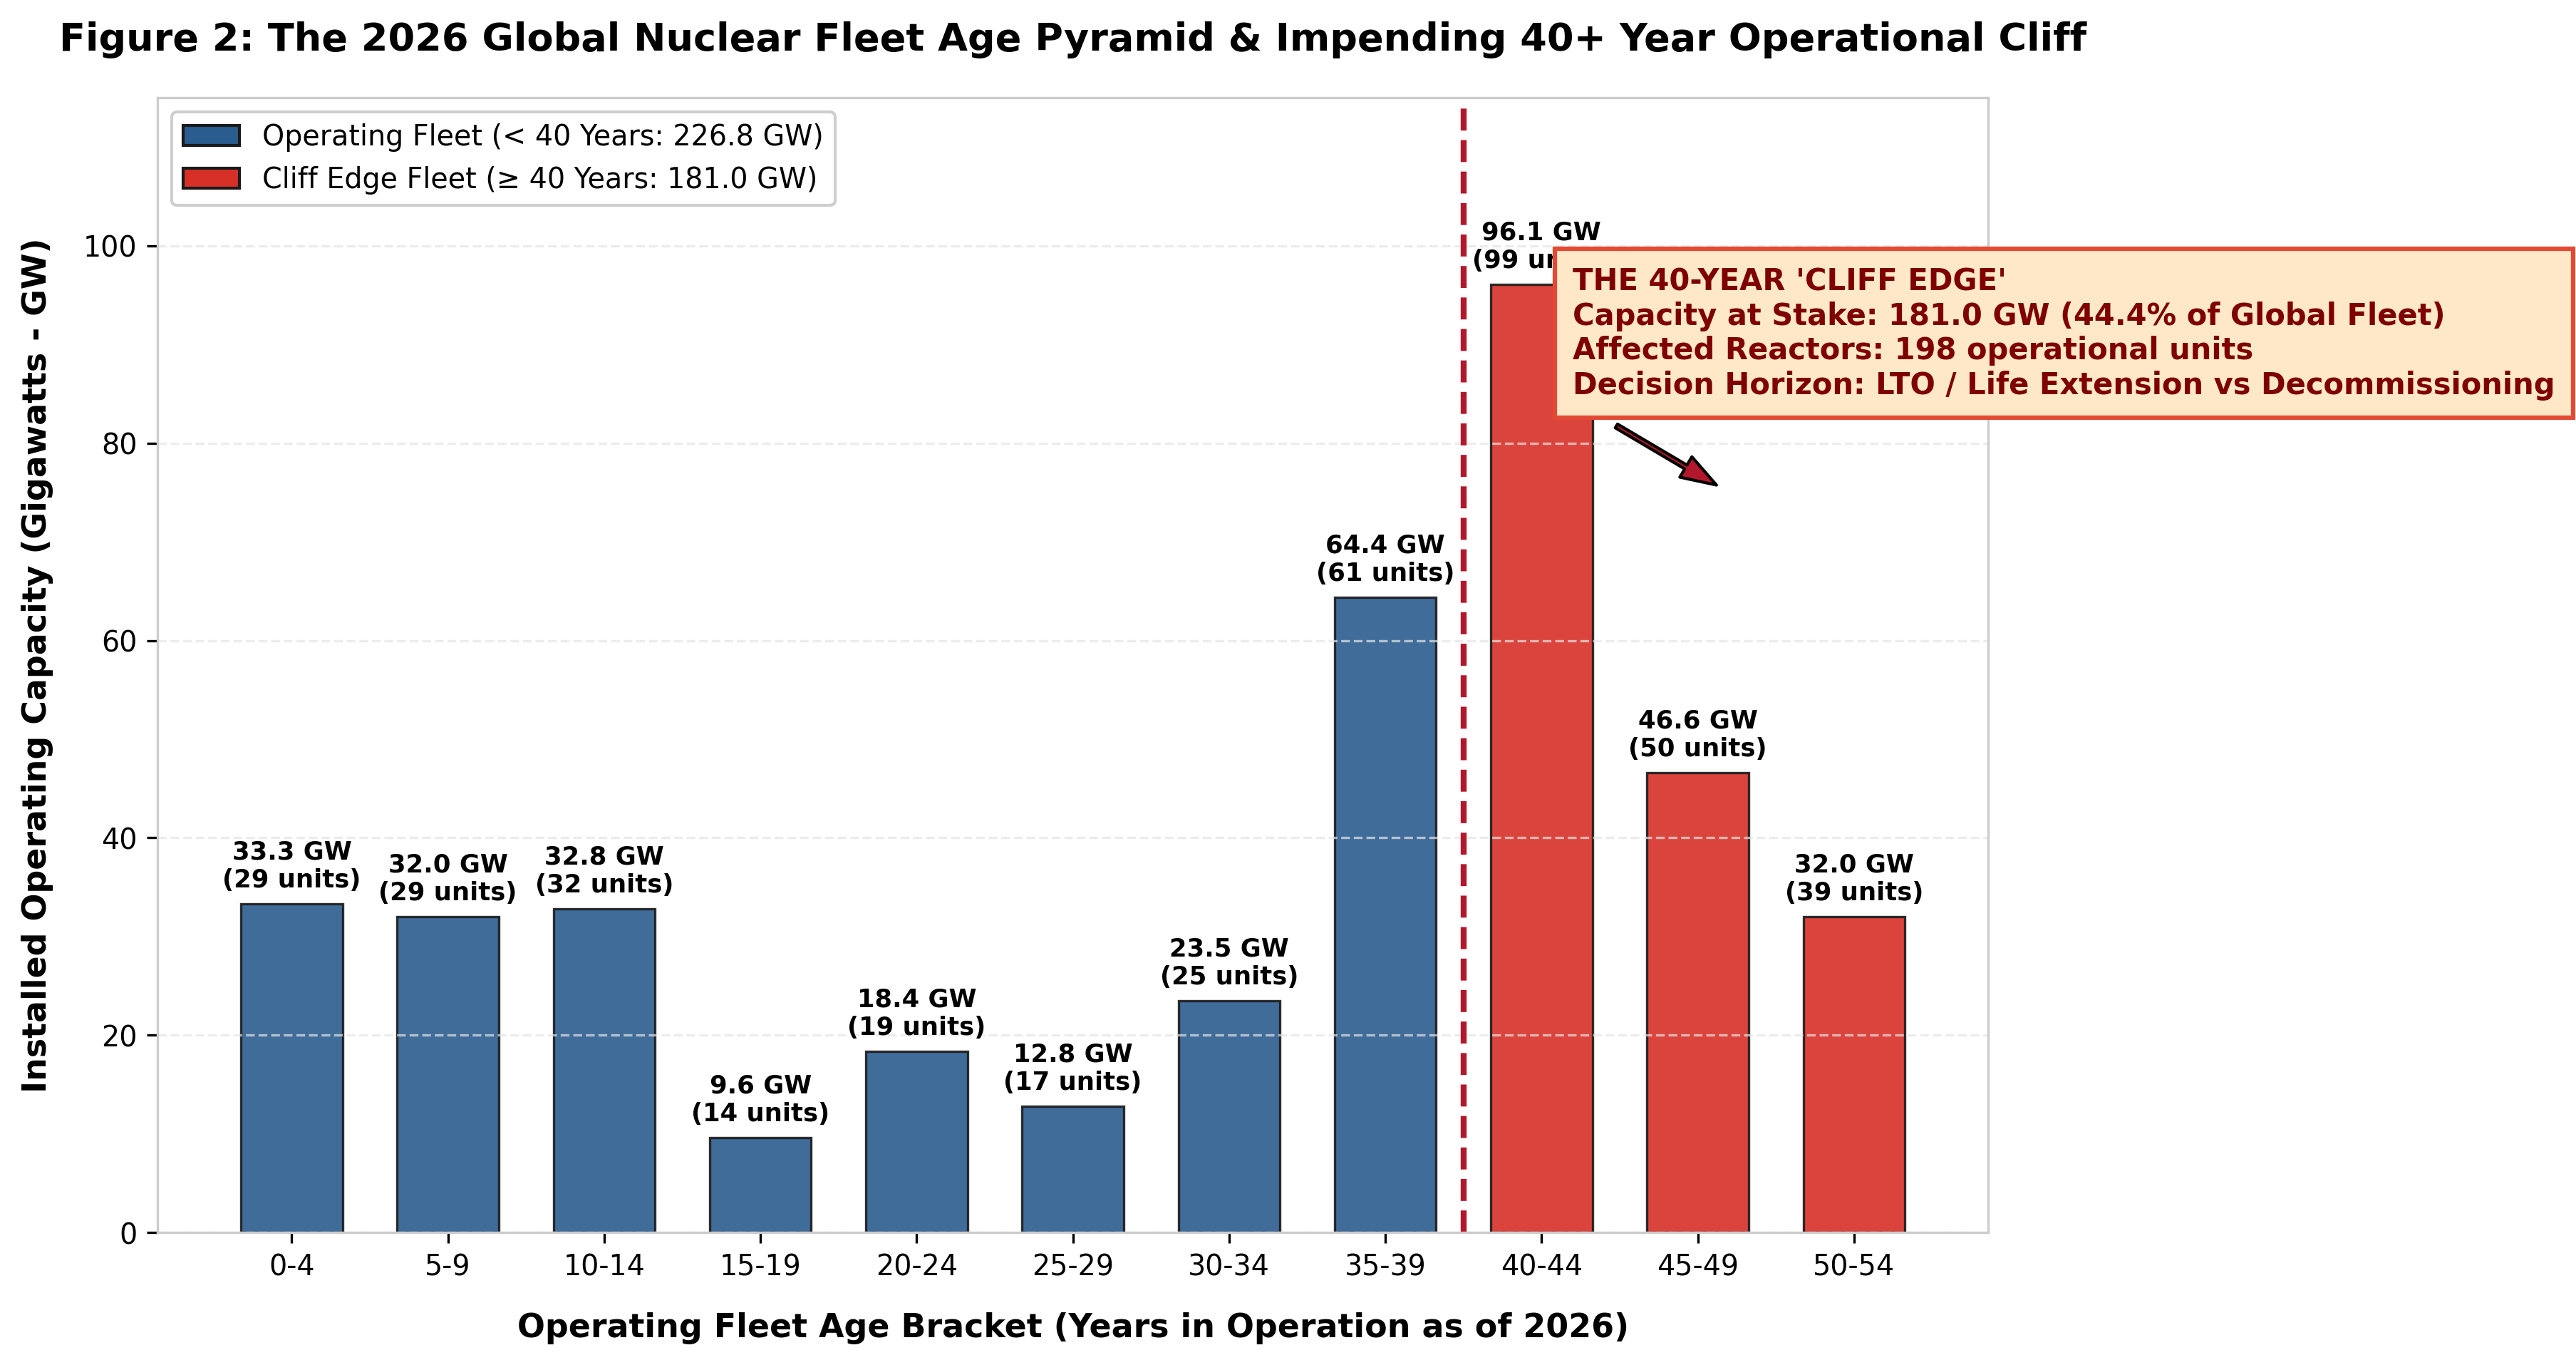
\includegraphics[width=\columnwidth]{fig2_nuclear_age_pyramid_cliff.png}
\caption{The 2026 Global Nuclear Fleet Age Pyramid highlighting the 40+ year operational cliff edge (181.0\,GW across 198 operational units).}
\label{fig:age_cliff}
\end{figure}

\subsection{The 40-Year Operational ``Cliff Edge''}
Evaluating the operational vintage of active reactors as of 2026:
\begin{equation}
\text{Age}_{2026} = 2026 - \text{Start Year}
\end{equation}
As illustrated in \cref{fig:age_cliff}, \textbf{198 operating reactors} have attained or exceeded 40 years of commercial service. These units represent \textbf{180.99\,GW}, or \textbf{44.38\% of global operating nuclear capacity}. Geographically, this aging fleet is concentrated in North America (78 units, 76.4\,GW), Western Europe (64 units, 62.1\,GW), and Eastern Asia (38 units, 31.8\,GW). Without synchronized capital reinvestment (LTO), global power grids face an unprecedented supply shock by 2035.

\subsection{Empirical Construction Lead Times}
We compute historical construction durations:
\begin{equation}
\Delta t_{\text{lead}} = \frac{\text{COD} - \text{Construction Start Date}}{365.25}
\end{equation}
Across operating units, the empirical mean construction duration is \textbf{8.76 years} (median: \textbf{7.16 years}, IQR: [5.66, 10.18], standard deviation: 5.32 years). As depicted in \cref{fig:durations}, Pressurized Water Reactors (PWR, $n=384$) exhibit a median of 7.14 years, while Boiling Water Reactors (BWR, $n=49$) show a median of 6.42 years. Significant geographical divergences emerge: Eastern Asia exhibits disciplined execution (median: 5.8 years), whereas Western Europe (median: 9.4 years) and North America (median: 10.2 years) display pronounced tail risks \cite{grubler2010french}.

\begin{figure}[t]
\centering
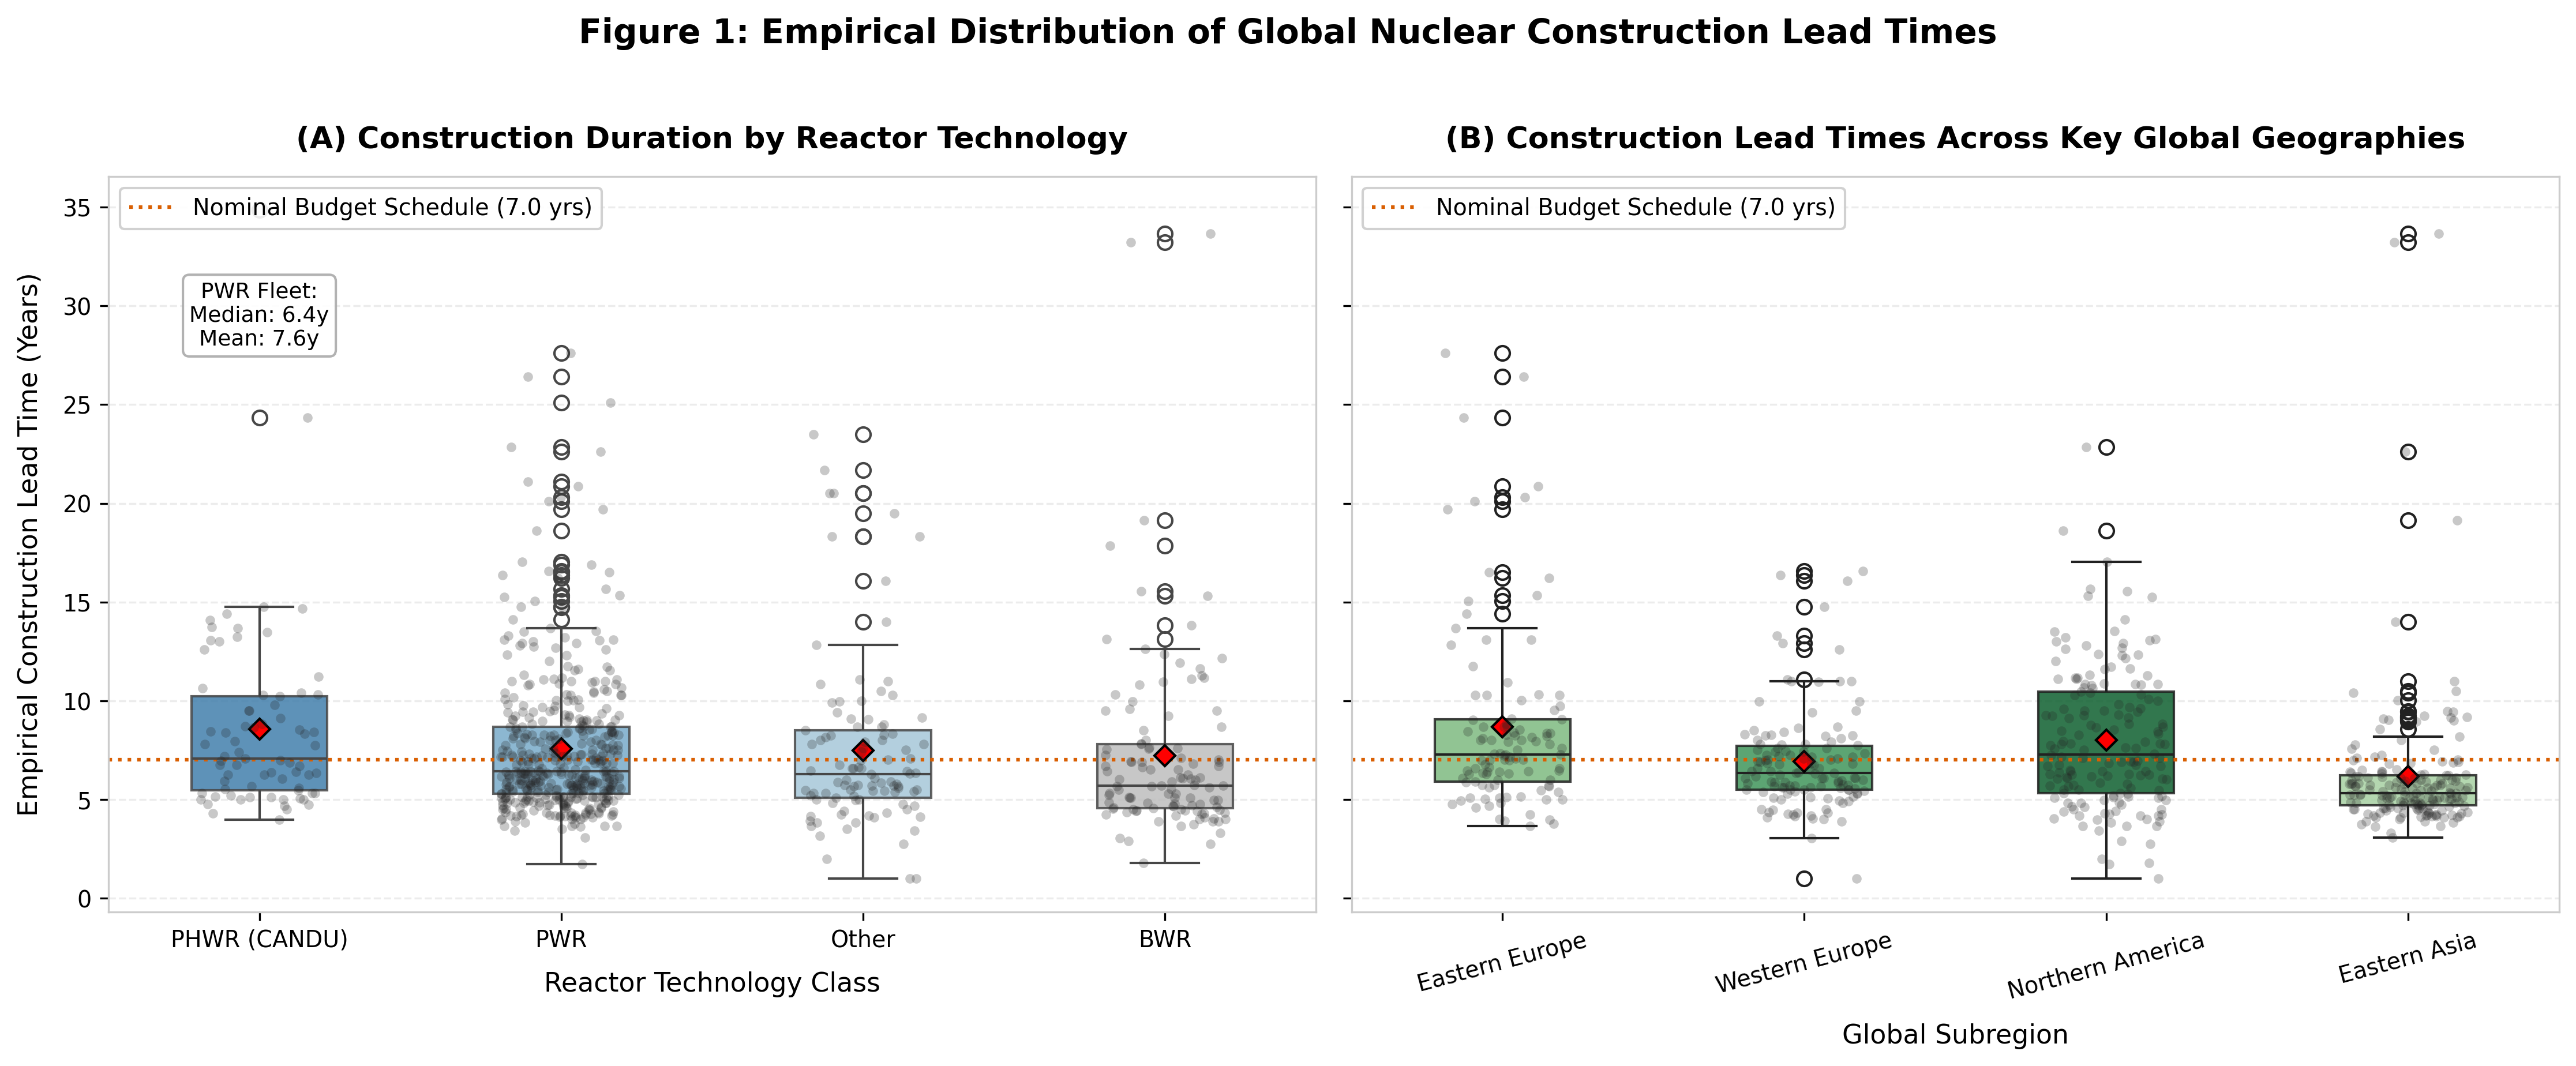
\includegraphics[width=\columnwidth]{fig1_construction_durations.png}
\caption{Empirical distribution of construction durations by reactor technology (A) and key geographic subregion (B).}
\label{fig:durations}
\end{figure}

\section{Quantitative Financial Methodology}
\subsection{Capital Expenditure Benchmarks}
Drawing on empirical benchmarks from the IEA/NEA \cite{iea2020projected} and EPRI \cite{epri2022lto}, we calibrate three distinct capital strategies:
\begin{itemize}
    \item \textbf{Gen-III+ (EPR/AP1000)}: $\text{Capex}_{\text{overnight}} = \$7,500/\text{kW}$, nominal construction duration $T_0 = 7.0$ years, operational economic lifetime $N = 60$ years.
    \item \textbf{Small Modular Reactor (SMR FOAK)}: $\text{Capex}_{\text{overnight}} = \$9,000/\text{kW}$, $T_0 = 4.0$ years, $N = 40$ years.
    \item \textbf{20-Year LTO (Grand Car{\'e}nage)}: $\text{Capex}_{\text{overnight}} = \$1,200/\text{kW}$, execution outage $T_0 = 2.0$ years, extended lifetime $N = 20$ years.
\end{itemize}

\subsection{S-Curve Spend Distribution}
Capital deployment follows an S-curve parameterized by a normalized Beta cumulative distribution function:
\begin{equation}
S(\tau) = I_\tau(\alpha, \beta) = \frac{\int_0^\tau u^{\alpha-1}(1-u)^{\beta-1}\mathrm{d}u}{\mathrm{B}(\alpha, \beta)}, \quad \tau = \frac{t}{T} \in [0, 1]
\label{eq:scurve}
\end{equation}
where $\alpha = 2.5, \beta = 2.5$. The discrete annual disbursement fraction for year $t \in \{1, \dots, T\}$ is $w_t = S(t/T) - S((t-1)/T)$ such that $\sum_{t=1}^T w_t = 1.0$.

For delayed schedules ($T = T_0 + \Delta t$), fixed site carrying costs and project management overhead incur a cost escalation $\lambda = 1.5\%$ per year of delay:
\begin{equation}
\text{Capex}_{\text{esc}} = \text{Capex}_{\text{overnight}} \cdot (1 + \lambda \cdot \Delta t)
\end{equation}

\subsection{IDC Compounding Mechanics}
Interest During Construction compounds cash disbursements up to the Commercial Operation Date ($T$):
\begin{equation}
\text{Capex}_{\text{total}}(T, r) = \sum_{t=1}^{T} w_t \cdot \text{Capex}_{\text{esc}} \cdot (1 + r)^{T - t + 0.5}
\label{eq:idc}
\end{equation}
where $r$ is the project WACC under a mid-year discounting convention \cite{rothwell2016economics}. The IDC Multiplier is defined as $\text{Capex}_{\text{total}} / \text{Capex}_{\text{overnight}}$.

\subsection{Levelized Cost of Electricity (LCOE)}
The Levelized Cost of Electricity (\$/MWh) is formulated as:
\begin{equation}
\text{LCOE} = \frac{\text{CRF}(r, N) \cdot \text{Capex}_{\text{total}} + \text{Fixed O\&M}}{8760 \cdot \text{CF}} + \text{Var O\&M} + \text{Fuel}
\label{eq:lcoe}
\end{equation}
where the Capital Recovery Factor ($\text{CRF}$) is:
\begin{equation}
\text{CRF}(r, N) = \frac{r(1 + r)^N}{(1 + r)^N - 1}
\label{eq:crf}
\end{equation}
Capacity factors are set to $\text{CF} = 0.88$ for new builds and $\text{CF} = 0.85$ for LTO (accounting for extended quadrennial inspections). Fixed O\&M is set to \$110/kW-yr for Gen-III+, \$125/kW-yr for SMR, and \$135/kW-yr for LTO.

\begin{figure}[t]
\centering
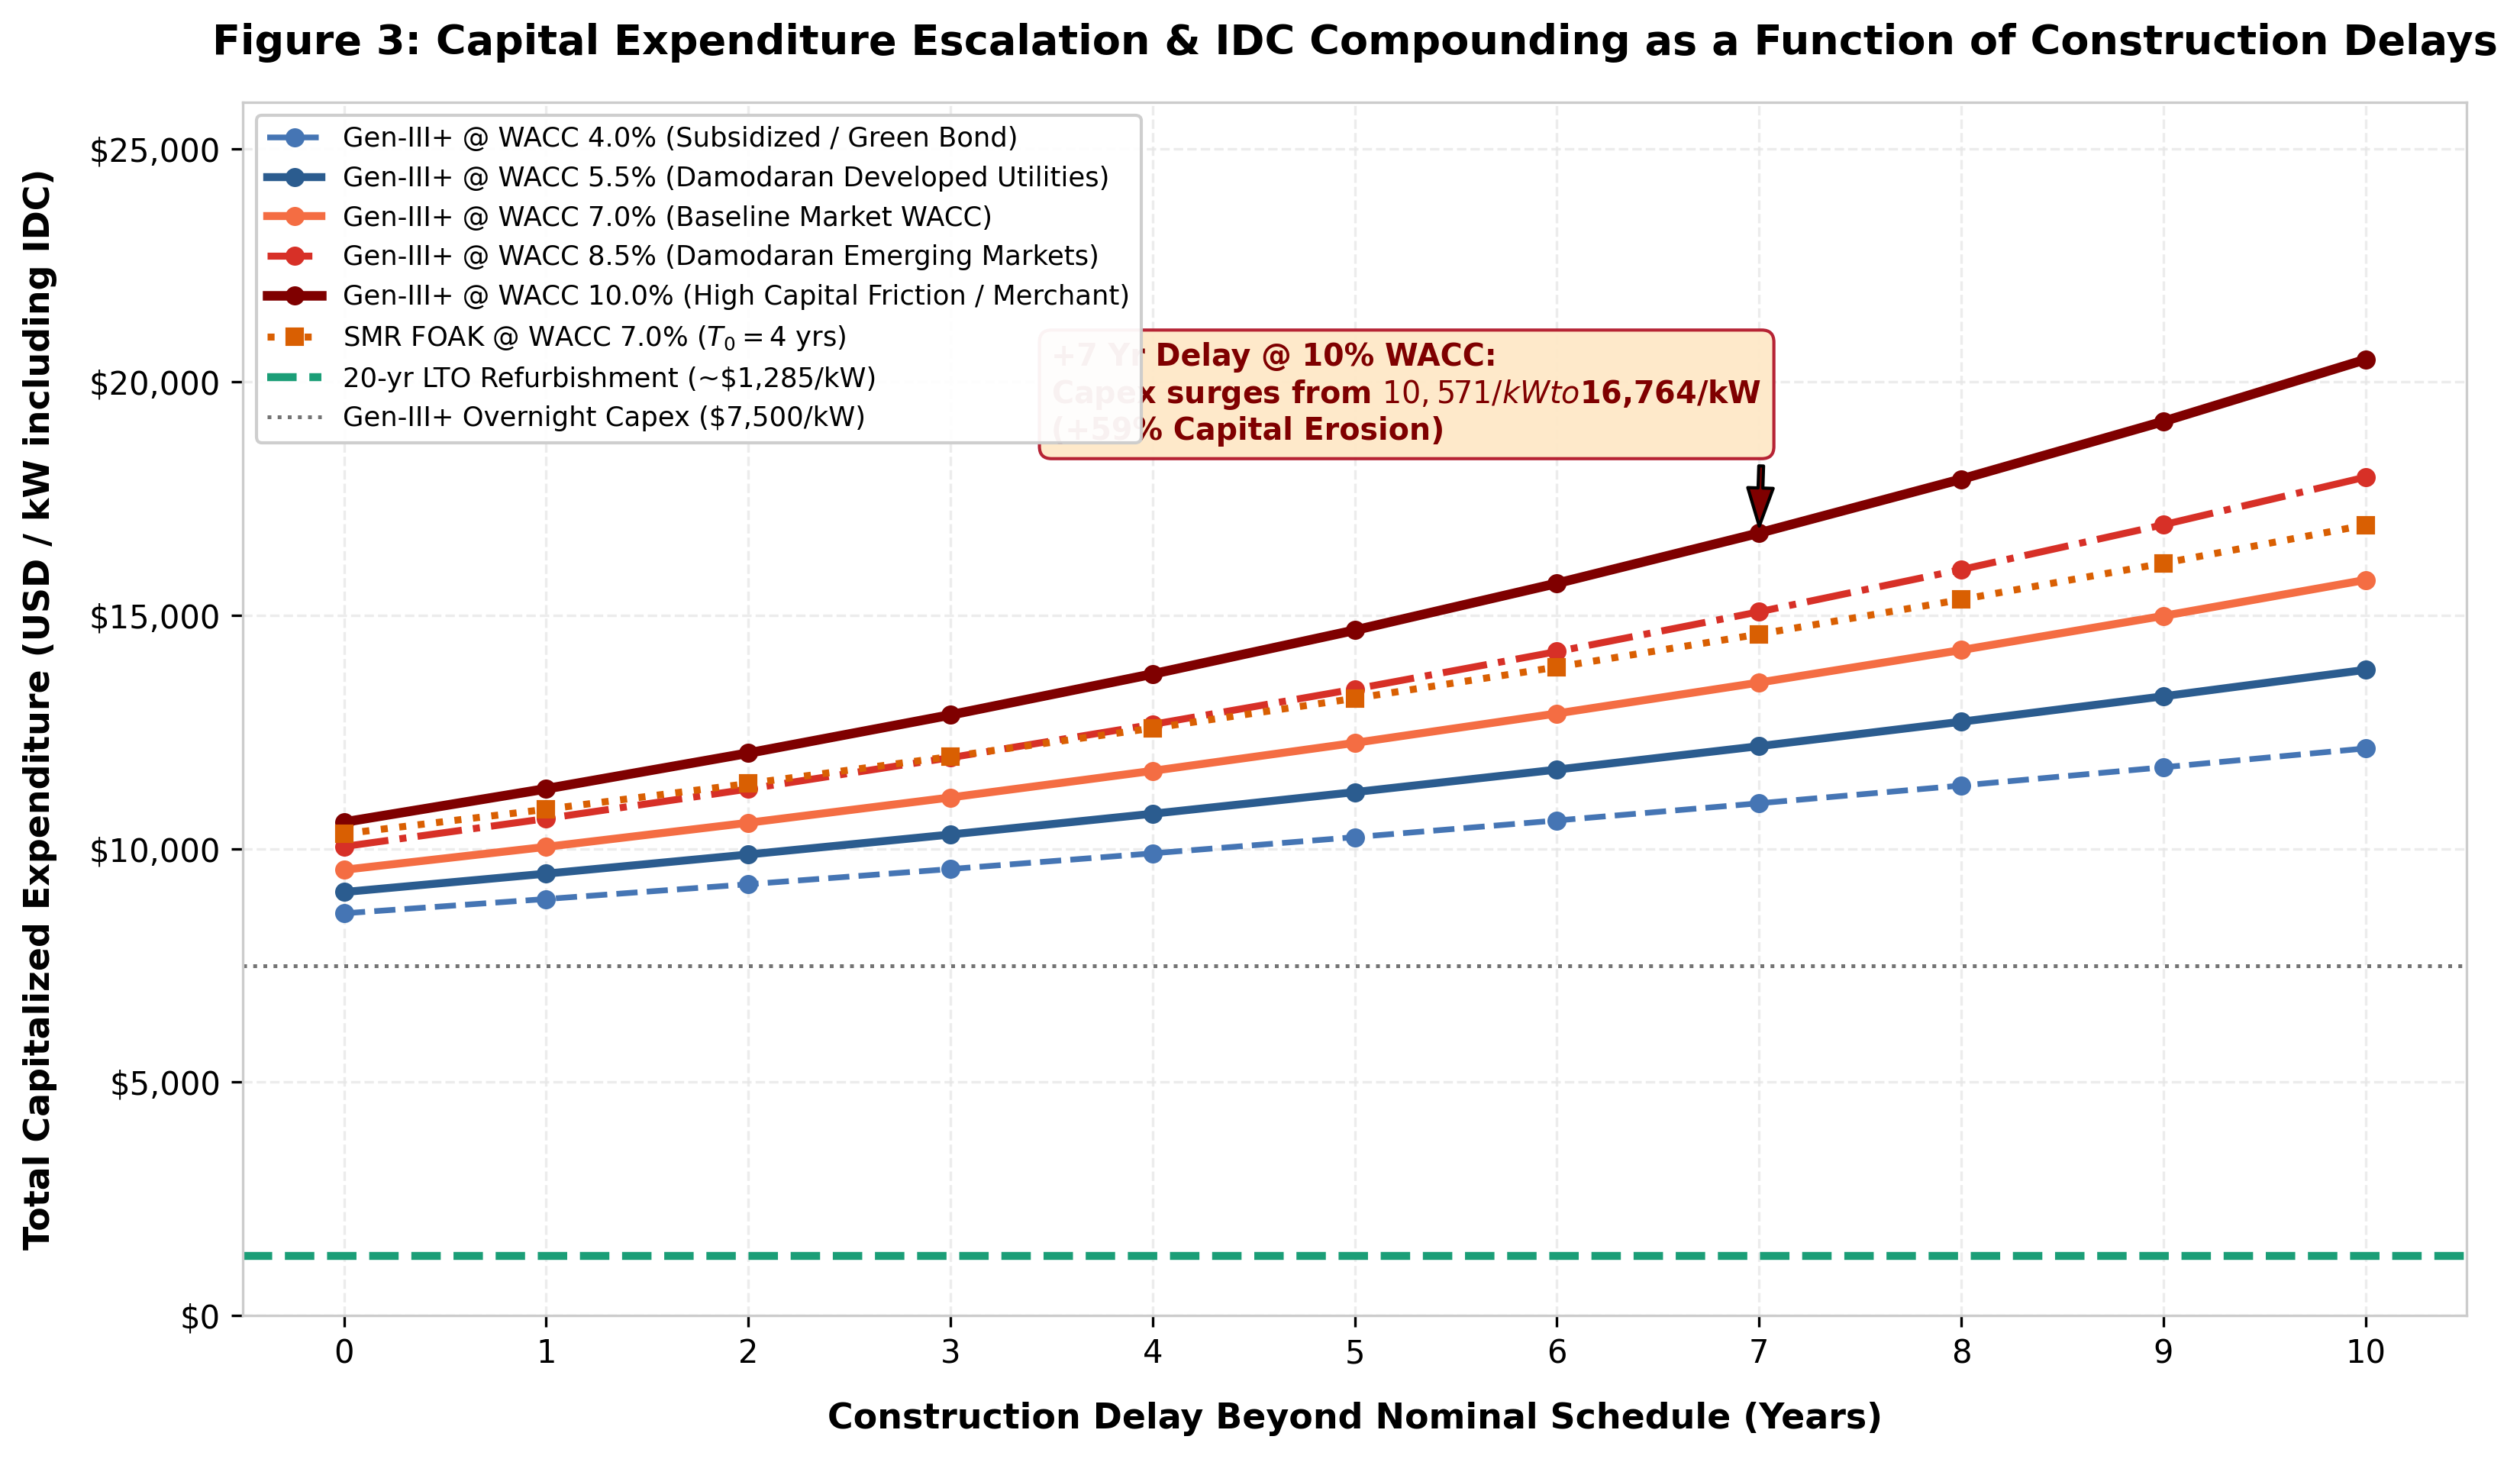
\includegraphics[width=\columnwidth]{fig3_idc_compounding_escalation.png}
\caption{Compounded capital expenditure ($\text{Capex}_{\text{total}}/\text{kW}$) as a function of construction delays across WACC regimes.}
\label{fig:idc_curve}
\end{figure}

\section{Empirical Results \& Sensitivity}
\subsection{IDC Compounding and Capital Escalation}
\cref{fig:idc_curve} and \cref{tab:capex_sensitivity} quantify the compounding of capital as lead times lengthen. At a baseline 7.0\% WACC, completing a Gen-III+ unit on its nominal 7-year schedule yields a capitalized cost of \$9,335/kW (+24.5\% IDC). When delays extend construction by 5 years (12-year COD), total capex surges to **\$12,713/kW** (+69.5\% IDC). Under high-friction merchant financing (10.0\% WACC) with a 7-year delay (14-year COD), capitalized cost reaches **\$17,358/kW** (+131.4\% IDC).

\begin{table}[b]
\centering
\small
\caption{Gen-III+ Total Capitalized Capex (\$/kW) across Delays and WACC}
\label{tab:capex_sensitivity}
\begin{tabularx}{\columnwidth}{lccccc}
\toprule
\textbf{Delay ($\Delta t$)} & \textbf{4.0\%} & \textbf{5.5\%} & \textbf{7.0\%} & \textbf{8.5\%} & \textbf{10.0\%} \\
\midrule
+0 yrs (7y COD)  & \$8,468  & \$8,890  & \$9,335  & \$9,804  & \$10,297 \\
+2 yrs (9y COD)  & \$9,198  & \$9,819  & \$10,488 & \$11,207 & \$11,983 \\
+4 yrs (11y COD) & \$9,985  & \$10,845 & \$11,791 & \$12,832 & \$13,979 \\
+6 yrs (13y COD) & \$10,832 & \$11,987 & \$13,287 & \$14,752 & \$16,403 \\
+8 yrs (15y COD) & \$11,745 & \$13,260 & \$15,007 & \$17,020 & \$19,343 \\
+10 yrs (17y COD)& \$12,731 & \$14,682 & \$16,988 & \$19,701 & \$22,897 \\
\bottomrule
\end{tabularx}
\end{table}

Conversely, 20-year LTO exhibits negligible compounding: overnight expenditure of \$1,200/kW results in a capitalized total of \$1,248/kW at 4.0\% WACC and \$1,348/kW at 10.0\% WACC, buffering utilities against macro-rate volatility.

\begin{figure}[t]
\centering
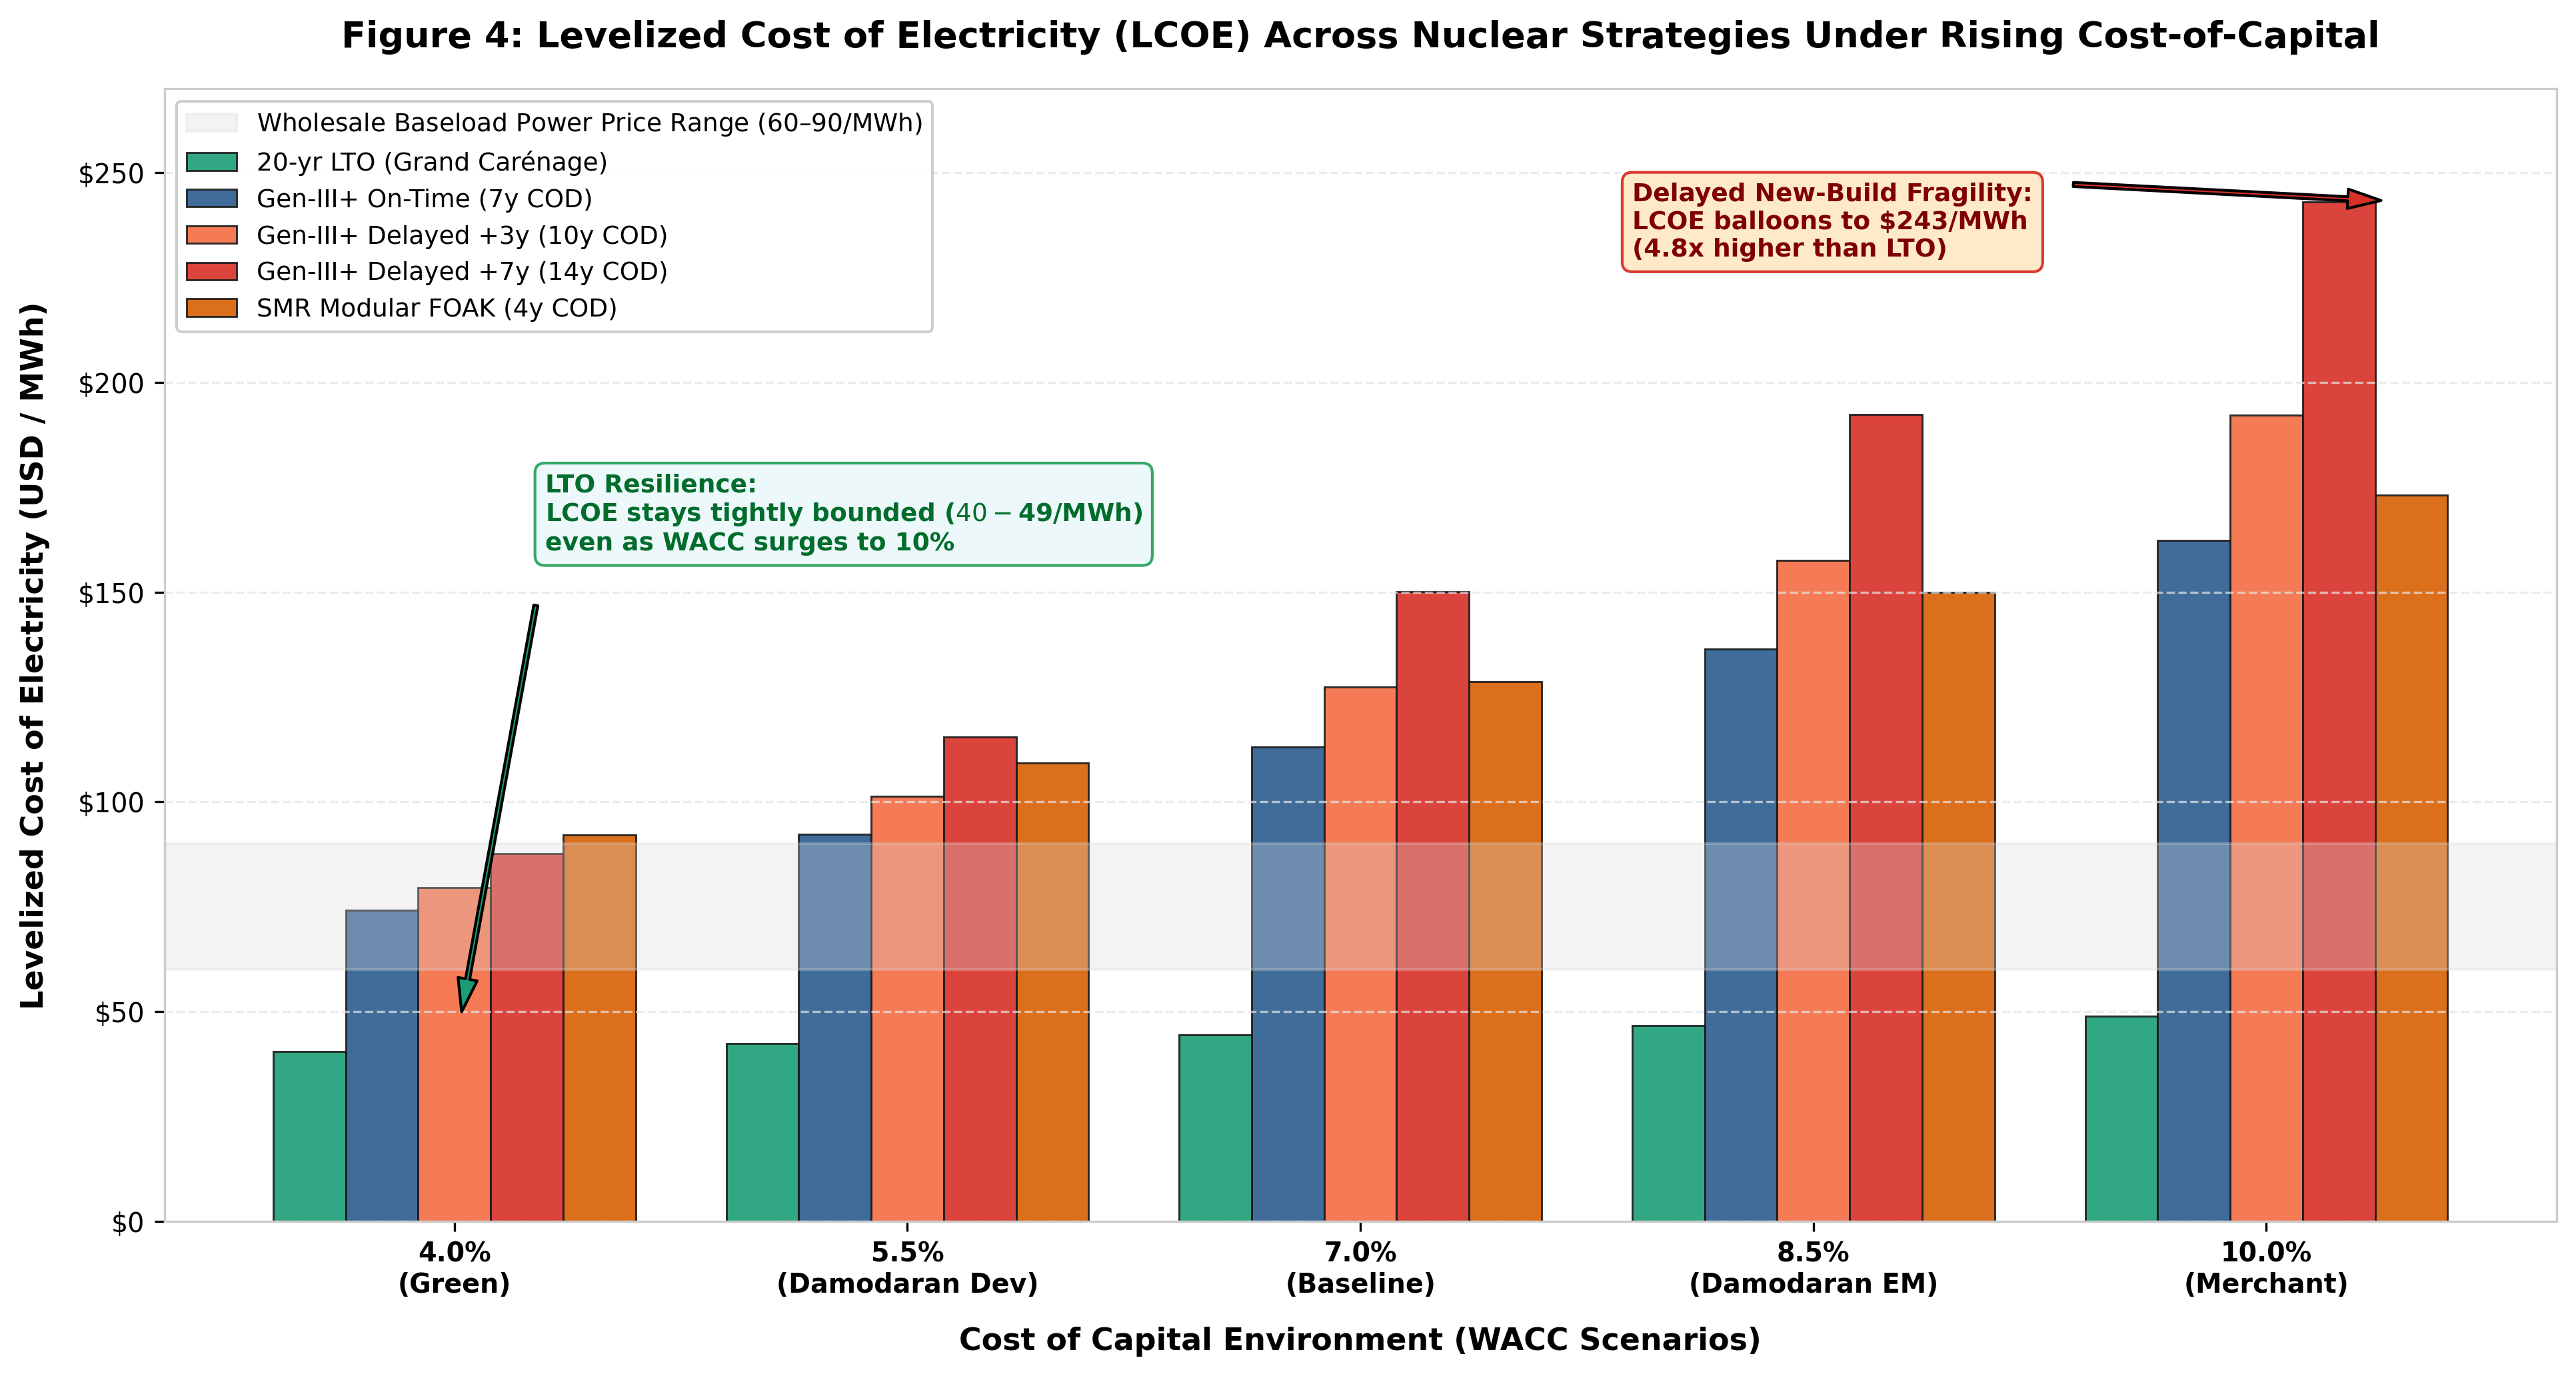
\includegraphics[width=\columnwidth]{fig4_lcoe_comparison_lto_vs_newbuild.png}
\caption{LCOE comparison across nuclear asset strategies and WACC regimes relative to wholesale baseload power price benchmarks.}
\label{fig:lcoe_chart}
\end{figure}

\begin{table*}[t]
\centering
\small
\caption{Levelized Cost of Electricity (\$/MWh) and Comparative Multipliers Relative to 20-Year LTO}
\label{tab:lcoe_comp}
\begin{tabularx}{\textwidth}{lccccc ccccc}
\toprule
& \multicolumn{5}{c}{\textbf{Levelized Cost of Electricity (\$/MWh)}} & \multicolumn{5}{c}{\textbf{Cost Ratio Relative to LTO (Gen-III+ / LTO)}} \\
\cmidrule(lr){2-6} \cmidrule(lr){7-11}
\textbf{Investment Strategy} & \textbf{4.0\%} & \textbf{5.5\%} & \textbf{7.0\%} & \textbf{8.5\%} & \textbf{10.0\%} & \textbf{4.0\%} & \textbf{5.5\%} & \textbf{7.0\%} & \textbf{8.5\%} & \textbf{10.0\%} \\
\midrule
\textbf{20-Year LTO (On-Time)}      & \textbf{\$40.47} & \textbf{\$42.34} & \textbf{\$44.42} & \textbf{\$46.66} & \textbf{\$48.98} & 1.00$\times$ & 1.00$\times$ & 1.00$\times$ & 1.00$\times$ & 1.00$\times$ \\
Gen-III+ On-Time (7y COD)           & \$74.18          & \$92.17          & \$113.01         & \$136.42         & \$162.35         & 1.83$\times$ & 2.18$\times$ & 2.54$\times$ & 2.92$\times$ & 3.31$\times$ \\
Gen-III+ Delayed +3y (10y COD)      & \$79.62          & \$101.48         & \$127.33         & \$157.69         & \$192.25         & 1.90$\times$ & 2.40$\times$ & 2.71$\times$ & 3.15$\times$ & 3.60$\times$ \\
Gen-III+ Delayed +5y (12y COD)      & \$83.54          & \$108.31         & \$138.14         & \$174.11         & \$215.86         & 2.00$\times$ & 2.56$\times$ & 2.94$\times$ & 3.48$\times$ & 4.04$\times$ \\
Gen-III+ Delayed +7y (14y COD)      & \$87.71          & \$115.65         & \$149.97         & \$192.36         & \$242.42         & 2.10$\times$ & 2.73$\times$ & 3.19$\times$ & 3.84$\times$ & 4.54$\times$ \\
SMR Modular FOAK (4y COD)           & \$92.05          & \$109.11         & \$128.65         & \$150.48         & \$173.17         & 2.27$\times$ & 2.58$\times$ & 2.90$\times$ & 3.22$\times$ & 3.54$\times$ \\
\bottomrule
\end{tabularx}
\end{table*}

\subsection{LCOE Superiority of Fleet Life Extension}
\cref{fig:lcoe_chart} and \cref{tab:lcoe_comp} present the central economic conclusion:
\begin{enumerate}
    \item \textbf{LTO Price Invariance}: Across all capital costs, 20-year LTO generates electricity between **\$40.47 and \$48.98/MWh**, clearing wholesale market baseload price ranges (\$60--\$90/MWh) with positive economic rent.
    \item \textbf{New-Build Cost Penalty}: On-time Gen-III+ requires \$113.01/MWh at 7.0\% WACC (2.54$\times$ LTO). With a 5-year delay, generation costs rise to \$138.14/MWh (2.94$\times$ LTO).
    \item \textbf{The Merchant Rate Trap}: Under private merchant equity hurdles (10.0\% WACC), Gen-III+ generation costs escalate to \$162.35/MWh on-time and \$215.86/MWh with a 5-year delay. SMRs produce electricity at \$128.65/MWh on-time at 7\% WACC, failing to match LTO economics prior to extensive series factory learning.
\end{enumerate}

\section{Strategic Recommendations}
\subsection{Asset Portfolio Sequencing}
Utilities facing capital allocation decisions must enforce an **``LTO First'' sequence**. Refurbishing the 181.0\,GW of mature reactors requires \$217 billion in capital, compared to \$1.36 trillion required to build equivalent Gen-III+ replacement capacity. LTO preserves vital grid inertia and zero-carbon baseload at an average capital saving of over **\$1.1 trillion**.

\subsection{Financing Instruments: Mitigating Debt Compounding}
Private capital markets cannot absorb greenfield nuclear construction risk under merchant pricing. To achieve investment viability, policy frameworks must compress WACCs below 5.0\%:
\begin{itemize}
    \item \textbf{Regulated Asset Base (RAB)}: Allowing utilities to charge consumers during the construction phase removes IDC accumulation and lowers capital costs by 30--45\% (e.g., UK Sizewell C).
    \item \textbf{Contracts for Difference (CfD)}: Index-linked revenue floors eliminate wholesale price volatility.
    \item \textbf{Green Taxonomy Inclusion}: Eligibility under the EU Sustainable Finance Taxonomy lowers debt risk spreads by 30--60 bps.
\end{itemize}

\section{Data Integration \& Research Extensions}
To expand this model, future empirical iterations will integrate:
\begin{enumerate}
    \item \textbf{Host-Country WACC Tables \cite{damodaran2026wacc}}: Linking sovereign credit risk to regional nuclear project financing (5.5\% in US/EU vs. 8.5--10.0\% in emerging markets).
    \item \textbf{IEA WEO Learning Rates}: Modeling SMR Capex learning curves as cumulative manufactured capacity scales.
    \item \textbf{IAEA PRIS Availability Databases}: Incorporating empirical forced outage rates for reactors operating beyond 50 years.
\end{enumerate}

\section{Conclusion}
Long-Term Operation (LTO) is the most capital-efficient, low-risk decarbonization instrument available in global power systems. Greenfield new builds and SMRs face severe debt compounding and capital erosion under realistic schedule slippages. Preserving the 181\,GW of nuclear assets approaching the 40-year cliff must be the overriding operational priority for utilities and climate risk regulators.

\bibliographystyle{IEEEtran}
\bibliography{references}

\end{document}
